\documentclass[tikz, border=15pt]{standalone}
\usepackage{tikz}
\usetikzlibrary{calc, arrows.meta, positioning, shapes.geometric}

\definecolor{encbg}{HTML}{FFF5F5}
\definecolor{encborder}{HTML}{E53E3E}
\definecolor{decbg}{HTML}{EBF8FF}
\definecolor{decborder}{HTML}{3182CE}
\definecolor{mha}{HTML}{ED8936}
\definecolor{ffn}{HTML}{38A169}
\definecolor{addnorm}{HTML}{ECC94B}
\definecolor{embed}{HTML}{9F7AEA}

\begin{document}
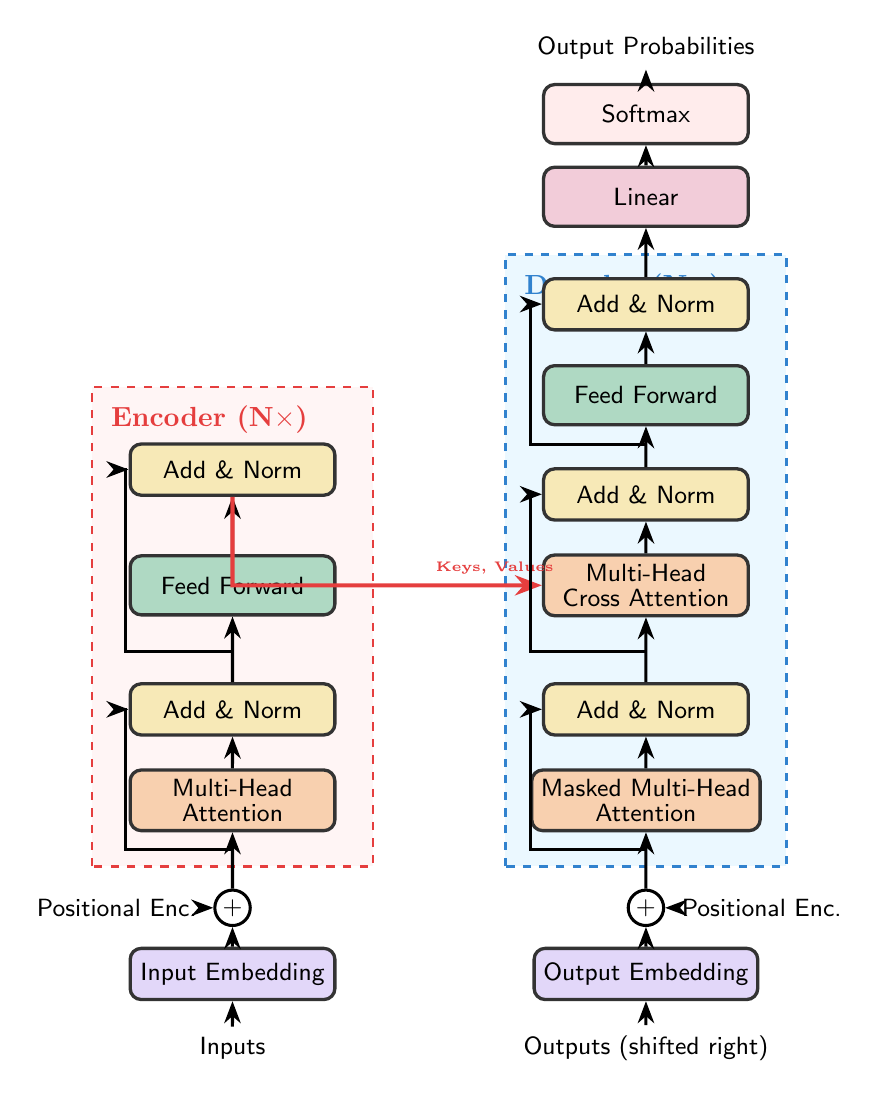
\begin{tikzpicture}[
    scale=1.05,
    >=Stealth,
    line width=1.1pt,
    font=\sffamily\small,
    block/.style={draw=black!80, fill=#1, rounded corners=4pt, line width=1.2pt, minimum width=2.6cm, minimum height=0.75cm, align=center},
    addnorm_style/.style={draw=black!80, fill=addnorm!40, rounded corners=4pt, line width=1.2pt, minimum width=2.6cm, minimum height=0.65cm, align=center},
    mha_style/.style={draw=black!80, fill=mha!40, rounded corners=4pt, line width=1.2pt, minimum width=2.6cm, minimum height=0.75cm, align=center},
    ffn_style/.style={draw=black!80, fill=ffn!40, rounded corners=4pt, line width=1.2pt, minimum width=2.6cm, minimum height=0.75cm, align=center},
    embed_style/.style={draw=black!80, fill=embed!30, rounded corners=4pt, line width=1.2pt, minimum width=2.6cm, minimum height=0.65cm, align=center},
    sum/.style={draw=black, circle, fill=white, inner sep=0pt, minimum size=0.45cm}
]

    % Encoder Stack Container Box (Left)
    \fill[encbg, draw=encborder, dashed, line width=1pt] (-4.5, 0.4) rectangle (-1.1, 6.2);
    \node[encborder, font=\bfseries, anchor=north west] at (-4.4, 6.1) {Encoder (N$\times$)};

    % Decoder Stack Container Box (Right)
    \fill[decbg, draw=decborder, dashed, line width=1pt] (0.5, 0.4) rectangle (3.9, 7.8);
    \node[decborder, font=\bfseries, anchor=north west] at (0.6, 7.7) {Decoder (N$\times$)};

    % --- ENCODER (Left Side) ---
    % Inputs & Embedding
    \node (in_text) at (-2.8, -1.8) {Inputs};
    \node[embed_style] (in_emb) at (-2.8, -0.9) {Input Embedding};
    \node[sum] (in_sum) at (-2.8, -0.1) {$+$};
    \node (in_pos) at (-4.2, -0.1) {Positional Enc.};

    % Encoder Stack Nodes
    \node[mha_style] (enc_mha) at (-2.8, 1.2) {Multi-Head\\[-2pt]Attention};
    \node[addnorm_style] (enc_an1) at (-2.8, 2.3) {Add \& Norm};
    \node[ffn_style] (enc_ffn) at (-2.8, 3.8) {Feed Forward};
    \node[addnorm_style] (enc_an2) at (-2.8, 5.2) {Add \& Norm};

    % Encoder Flow & Residual Connections
    \draw[->] (in_text) -- (in_emb);
    \draw[->] (in_emb) -- (in_sum);
    \draw[->] (in_pos) -- (in_sum);
    \draw[->] (in_sum) -- (enc_mha);

    % Residual 1 in Encoder
    \draw[->] (enc_mha) -- (enc_an1);
    \draw[->] (-2.8, 0.6) -- (-4.1, 0.6) |- (enc_an1);

    % Residual 2 in Encoder
    \draw[->] (enc_an1) -- (enc_ffn);
    \draw[->] (enc_ffn) -- (enc_an2);
    \draw[->] (-2.8, 3.0) -- (-4.1, 3.0) |- (enc_an2);


    % --- DECODER (Right Side) ---
    % Outputs & Embedding
    \node (out_text) at (2.2, -1.8) {Outputs (shifted right)};
    \node[embed_style] (out_emb) at (2.2, -0.9) {Output Embedding};
    \node[sum] (out_sum) at (2.2, -0.1) {$+$};
    \node (out_pos) at (3.6, -0.1) {Positional Enc.};

    % Decoder Stack Nodes
    \node[mha_style] (dec_mmha) at (2.2, 1.2) {Masked Multi-Head\\[-2pt]Attention};
    \node[addnorm_style] (dec_an1) at (2.2, 2.3) {Add \& Norm};
    \node[mha_style] (dec_cross) at (2.2, 3.8) {Multi-Head\\[-2pt]Cross Attention};
    \node[addnorm_style] (dec_an2) at (2.2, 4.9) {Add \& Norm};
    \node[ffn_style] (dec_ffn) at (2.2, 6.1) {Feed Forward};
    \node[addnorm_style] (dec_an3) at (2.2, 7.2) {Add \& Norm};

    % Linear & Softmax Output Layer
    \node[block=purple!20] (linear) at (2.2, 8.5) {Linear};
    \node[block=pink!30] (softmax) at (2.2, 9.5) {Softmax};
    \node (prob) at (2.2, 10.3) {Output Probabilities};

    % Decoder Flow & Residual Connections
    \draw[->] (out_text) -- (out_emb);
    \draw[->] (out_emb) -- (out_sum);
    \draw[->] (out_pos) -- (out_sum);
    \draw[->] (out_sum) -- (dec_mmha);

    % Residual 1 in Decoder
    \draw[->] (dec_mmha) -- (dec_an1);
    \draw[->] (2.2, 0.6) -- (0.8, 0.6) |- (dec_an1);

    % Cross Attention Connection from Encoder Output to Decoder
    \draw[->, line width=1.5pt, encborder] (enc_an2) |- (-0.2, 3.8) -- (dec_cross) node[midway, above, font=\tiny\bfseries] {Keys, Values};

    % Residual 2 in Decoder
    \draw[->] (dec_an1) -- (dec_cross);
    \draw[->] (dec_cross) -- (dec_an2);
    \draw[->] (2.2, 3.0) -- (0.8, 3.0) |- (dec_an2);

    % Residual 3 in Decoder
    \draw[->] (dec_an2) -- (dec_ffn);
    \draw[->] (dec_ffn) -- (dec_an3);
    \draw[->] (2.2, 5.5) -- (0.8, 5.5) |- (dec_an3);

    % Output Layer Flow
    \draw[->] (dec_an3) -- (linear);
    \draw[->] (linear) -- (softmax);
    \draw[->] (softmax) -- (prob);

\end{tikzpicture}
\end{document}
